\documentclass[sigconf]{acmart}

\usepackage{adjustbox}
\usepackage{algorithm}
\usepackage{algpseudocode}
\usepackage{pgfplots}
\pgfplotsset{compat=1.17}

\setcopyright{none}
\settopmatter{printacmref=false}
\acmConference[ACM]{ACM}{November, 2026}{Lisbon, PT}
\citestyle{acmauthoryear}

% Colour code used in the result tables, as in the summary table.
\definecolor{win}{RGB}{46,139,48}
\definecolor{tie}{RGB}{214,160,0}
\definecolor{loss}{RGB}{214,48,49}
\newcommand{\win}[1]{\textcolor{win}{#1}}
\newcommand{\tie}[1]{\textcolor{tie}{#1}}
\newcommand{\loss}[1]{\textcolor{loss}{#1}}
\newcommand{\pmsd}[2]{#1{\scriptsize$\,\pm\,$#2}}

\begin{document}

\title{Fewer False Deaths, Shorter Tails: Failure Detection and Request Routing for a Dynamo-Style Key-Value Store}

\author{Martim Baltazar}
\email{martimnunesbaltazar@gmail.com}

\renewcommand{\shortauthors}{Martim Baltazar}

\begin{abstract}
Dynamo-style key-value stores trade consistency for availability, but two parts of their design remain fragile. Failure detection relies on fixed timeouts, so packet loss or a slow node makes healthy nodes look dead, while longer timeouts delay the detection of real failures. Request handling sends every read to all replicas and spreads keys, not traffic, so one slow replica inflates tail latency and one popular key overloads its replicas. We build a complete Dynamo-style store with SWIM membership in a deterministic simulator and replace these two parts. Suspicion lasts longer when it is unconfirmed and shortens as independent nodes confirm it; reads go to the replicas that have answered fastest lately, are hedged when slow, avoid overloaded nodes, and spread hot keys over temporary extra replicas. Against a classic baseline on identical seeds and faults, false death verdicts at 20\% packet loss fall from 77.7 to 0.3 per run, the 99th-percentile latency with one slow node falls from 1338\,ms to 210\,ms, and a key receiving half of all traffic leaves the busiest node at 1.16$\times$ the average load instead of 2.25$\times$. The costs are about 0.5\,s slower failure detection on a clean network, 2\,s under high latency, and 5--8\,ms per request when nothing is wrong.
\end{abstract}

\begin{CCSXML}
<ccs2012>
<concept>
<concept_id>10010520.10010575</concept_id>
<concept_desc>Computer systems organization~Dependable and fault-tolerant systems and networks</concept_desc>
<concept_significance>500</concept_significance>
</concept>
<concept>
<concept_id>10002951.10002952.10003190.10003195</concept_id>
<concept_desc>Information systems~Parallel and distributed DBMSs</concept_desc>
<concept_significance>300</concept_significance>
</concept>
</ccs2012>
\end{CCSXML}

\ccsdesc[500]{Computer systems organization~Dependable and fault-tolerant systems and networks}
\ccsdesc[300]{Information systems~Parallel and distributed DBMSs}

\keywords{Key-Value Store, Failure Detection, Gossip Protocols, Tail Latency, Load Balancing}

\maketitle

\section{Introduction}

Dynamo-style key-value stores~\cite{decandia2007dynamo,lakshman2010cassandra} place every key on $N$ nodes of a consistent-hash ring~\cite{karger1997consistent}, let any node coordinate a request, and wait for $R$ of the $N$ replicas on a read and $W$ on a write. When replicas are unreachable they keep writing through stand-ins (sloppy quorum and hinted handoff) and later reconcile copies with read repair and Merkle-tree anti-entropy~\cite{merkle1987digital}. Concurrent writes are kept as siblings and ordered with vector clocks~\cite{mattern1989virtual}. Membership and failure detection are typically gossip-based, for example with SWIM~\cite{das2002swim}.

Two parts of this design remain fragile. First, \textbf{failure detection uses fixed timeouts}. Under packet loss or a slow node, healthy members miss deadlines and are declared dead; lengthening the timeout suppresses these false verdicts but delays the detection of real crashes. Second, \textbf{request handling ignores speed and load}. Every read is sent to all $N$ replicas and coordinators are chosen at random, so a request that lands on a slow node waits for it; and the ring spreads keys evenly but not traffic, so a single popular key saturates its $N$ owners.

The key insight is that both problems can be solved with information each node already has. A real crash is noticed by many probers at once, whereas a lost message is noticed by one; so the time a suspicion is allowed to last should depend on how many independent nodes confirm it. Likewise, every reply carries its own latency and the replying node's load; so the coordinator can prefer replicas that are fast and lightly loaded, ask another only when one is slow, and give a hot key extra replicas only while it is hot.

We implement a complete Dynamo-style store and both improvements in a deterministic simulator, and compare them against the classic design on identical seeds, faults and workloads. The main contributions of this work are:
\begin{enumerate}
  \item A Dynamo-style store with SWIM membership, sloppy quorums, hinted handoff, vector clocks, read repair and Merkle anti-entropy, running in a deterministic, replayable simulator, used as the classic baseline.
  \item Agreement-based suspicion and phi-accrual probing for the membership layer, and load- and latency-aware read routing with hedging and temporary hot-key replicas for the coordinator.
  \item An evaluation over many seeds, with ablations that identify which mechanism produces each gain and which ones do not help.
\end{enumerate}

\section{Problem Statement}

Next, we present the notation adopted in the paper and formulate the problems in terms of research goals \textbf{RG}$_1$--\textbf{RG}$_3$.

\subsubsection{Notation.} We start by setting the notation adopted in this paper, summarized in Table~\ref{tab:notation}.

\begin{table}[h]
\caption{Notation used in this paper.}
\label{tab:notation}
\small
\begin{adjustbox}{max width=\columnwidth}
\begin{tabular}{|l|l|}
\hline
\textbf{Symbol} & \textbf{Description} \\ \hline
$\mathcal{V}$ & Set of storage nodes \\
$\mathcal{K}$ & Set of keys \\
$P(k)$ & Preference list: the $N$ distinct nodes owning key $k$ \\
$N, R, W$ & Replicas per key; replies needed to read; acks to write \\
$T_p$ & Protocol period: each node probes one member per period \\
$T_s$ & Suspicion timeout of the classic detector \\
$c$ & Independent confirmations of a suspicion \\
$\tau(c)$ & Suspicion timeout after $c$ confirmations \\
$\hat{\ell}_j$ & Coordinator's latency estimate for node $j$ \\
$L_j, \bar{L}$ & Load of node $j$; mean load over nodes \\
$\alpha$ & Load cap, as a multiple of $\bar{L}$ \\
$\lambda_k$ & Read rate of key $k$ observed by an owner \\
$p_{99}$ & 99th-percentile client latency \\ \hline
\end{tabular}
\end{adjustbox}
\end{table}

\subsubsection{Problem Formulation.} The problem we aim to solve is to change the failure detector and the coordinator of a Dynamo-style store so that it satisfies the following research goals:
\begin{description}
  \item[\textbf{RG}$_1$] \textit{Accurate failure detection:} Declare far fewer healthy nodes dead under packet loss and slow nodes, while detecting real crashes about as fast as the classic detector.
  \item[\textbf{RG}$_2$] \textit{Short tails:} Keep $p_{99}$ close to the median when one node is slow, without failing more requests.
  \item[\textbf{RG}$_3$] \textit{Balanced load at low cost:} Keep the busiest node within $\alpha\bar{L}$ under skewed and sudden hot-key workloads, without extra traffic, extra latency of note, or weaker consistency than the classic store.
\end{description}

In what follows, we propose a solution to the problem above and evaluate how the proposal satisfies \textbf{RG}$_1$--\textbf{RG}$_3$ in simulated experiments.

\section{The Proposed System}

Here, we describe the classic store we start from and the two changes we make to it. Every node runs SWIM~\cite{das2002swim}: each protocol period it pings one member, asks $k$ others to probe indirectly if no ack arrives, marks the member \emph{suspect} at the end of the period, and declares it \emph{dead} after $T_s$ unless the member refutes by gossiping a higher incarnation number. Membership updates are piggybacked on probe traffic. Ring membership is explicit: a dead verdict never changes $P(k)$; it only makes coordinators skip the node and, with sloppy quorum, hand its writes to the next live node as a hint.

\subsection{Agreement-Based Suspicion}

A suspicion started by node $i$ carries the identity of the node that failed to reach the member. Every other node that independently fails to reach it gossips a \emph{confirmation}. The suspicion timeout starts at $m\,T_s$ and falls logarithmically to $T_s$ as confirmations arrive:
\begin{equation}
\tau(c) = m\,T_s - (m-1)\,T_s \cdot \min\!\Big(1, \frac{\ln(c+1)}{\ln(K+1)}\Big),
\end{equation}
where $K$ is the number of confirmations needed to reach the minimum. This rule follows the dynamic suspicion timeout of Lifeguard~\cite{dadgar2018lifeguard}. We use $m=4$ and $K=2$. The procedure is outlined in Algorithm~\ref{alg:suspicion}. In addition, each node replaces SWIM's fixed ping timeout per peer with a phi-accrual timeout~\cite{hayashibara2004phi}: it waits until a reply would be later than $10^{-\varphi}$ of that peer's recent round trips, with $\varphi = 6$.

\begin{algorithm}[t]
\caption{Agreement-Based Suspicion at node $i$}
\label{alg:suspicion}
\begin{algorithmic}[1]
\Require Suspect timeout $T_s$, multiplier $m$, confirmations $K$
\Procedure{OnSuspect}{$j$, inc, by}
  \If{$j$ is alive at inc in $i$'s view}
    \State $s_j \gets (\text{start} = now,\ B = \{\text{by}\})$
    \State $d_j \gets now + \tau(0)$ \Comment{$= m\,T_s$}
    \State schedule \Call{Expire}{$j$} at $d_j$
  \ElsIf{$j$ is suspect at inc \textbf{and} by $\notin B$}
    \State $B \gets B \cup \{\text{by}\}$ \Comment{Independent confirmation}
    \State gossip the confirmation if $|B| \le K+1$
    \State $d_j \gets \min\big(d_j,\ \text{start} + \tau(|B|-1)\big)$
    \State schedule \Call{Expire}{$j$} at $\max(d_j, now)$
  \EndIf
\EndProcedure
\Procedure{Expire}{$j$}
  \If{$j$ still suspect at the same inc \textbf{and} $now \ge d_j$}
    \State declare $j$ dead and gossip the verdict
  \EndIf
\EndProcedure
\end{algorithmic}
\end{algorithm}

\subsection{Load- and Latency-Aware Reads}

The coordinator keeps a latency estimate $\hat{\ell}_j$ per node, updated as $\hat{\ell}_j \gets 0.8\,\hat{\ell}_j + 0.2\,x$ for each reply time $x$. A node that has not replied after waiting $w$ is recorded as $\hat{\ell}_j \gets \max(\hat{\ell}_j, w)$, so a node whose replies always arrive too late cannot look fast; estimates halve every 20\,s so slow nodes are retried. Every reply also reports the replier's load $L_j$, its replica operations per second. Algorithm~\ref{alg:read} shows how a read is served. Clients choose coordinators by the same latency rule and hedge a slow read through a second coordinator. Writes are never hedged, since a duplicated write would create a second version.

\textbf{Hot keys.} Each owner tracks $\lambda_k$ for the keys it serves. Above a threshold $\theta$ it lends the current value to the next $e$ nodes on the ring, where $e$ is sized so that each replica serves about $\theta$ reads per second:
\begin{equation}
e = \min\!\Big(E,\ |\mathcal{V}|-N,\ \max\!\big(1, \big\lceil \lambda_k (N+e')/\theta \big\rceil - N\big)\Big),
\end{equation}
with $e'$ the current number of extra replicas and $E$ a cap. Writes refresh lent copies immediately; copies lapse after 3\,s, and the key stops being hot when $\lambda_k < \theta/4$. We use $\theta = 20$ reads/s and $\alpha = 1.25$.

\begin{algorithm}[t]
\caption{Read of key $k$ at a coordinator}
\label{alg:read}
\begin{algorithmic}[1]
\Require $P(k)$, quorum $R$, estimates $\hat{\ell}$, loads $L$, cap $\alpha$
\State $C \gets$ the $N$ planned nodes: $P(k)$, with a stand-in for each owner declared dead
\If{$k$ is hot}
  \State $C \gets C \cup \{\text{its } e \text{ extra replicas}\}$; shuffle $C$
  \State move nodes with $L_j > \alpha\bar{L}$ to the end of $C$
\Else
  \State sort $C$ by $\hat{\ell}_j \cdot (1 + 0.2\,u_j) \cdot (2 \text{ if } L_j > \alpha\bar{L} \text{ else } 1)$ \Comment{$u_j \sim U(0,1)$}
\EndIf
\State send the read to the first $R$ nodes of $C$
\While{fewer than $R$ replies}
  \If{no reply after $2 \cdot \max \hat{\ell}$ of the nodes asked}
    \State send the read to the next node of $C$ \Comment{Hedge}
  \EndIf
\EndWhile
\State reply with the reconciled versions; read-repair stale owners
\end{algorithmic}
\end{algorithm}

\subsection{Theoretical Validation}

Next, we bound when a suspicion can end and how much extra traffic a read can send.

\begin{theorem}
A suspicion started at time $t_0$ and not refuted ends in a dead verdict at a time in $[t_0 + T_s,\ t_0 + m\,T_s]$. If at least $K$ confirmations arrive before $t_0 + T_s$, it ends at exactly $t_0 + T_s$.
\end{theorem}

\begin{proof}
$\tau$ is non-increasing in $c$, with $\tau(0) = m\,T_s$ and $\tau(c) = T_s$ for $c \ge K$, so $d_j$ always lies in $[t_0+T_s,\ t_0+m\,T_s]$. A verdict requires $now \ge d_j$, hence it cannot happen before $t_0 + T_s$. The timer scheduled at $t_0 + m\,T_s$ always finds $now \ge d_j$, hence the verdict happens by then. If $K$ confirmations arrive before $t_0 + T_s$, then $d_j = t_0 + \tau(K) = t_0 + T_s$ and a timer fires at that time.
\end{proof}

Hence the improved detector never declares a member dead earlier after a suspicion than the classic one, and at most $m$ times later.

\begin{theorem}
For a key that is not hot, a coordinator sends at most $N$ replica requests per read, as the classic store does, and a client sends each read to at most two coordinators.
\end{theorem}

\begin{proof}
Algorithm~\ref{alg:read} asks $R$ nodes and then at most one more per hedge, always from $C$, and $|C| \le N$ when $k$ is not hot. A client hedges a read at most once.
\end{proof}

\section{Experimental Results}

This section evaluates the proposed changes in terms of failure-detection accuracy and speed, tail latency, load balance and overhead. The code and scripts used to reproduce the experiments reported in this study are publicly available at the project repository: \url{https://github.com/MartimBaltazar/Dynamo-KV-store}.

\subsection{Research Questions}
In this section, we evaluate the proposed system with respect to the research goals outlined in Section~2. Specifically, we investigate the following research questions:
\begin{description}
  \item[\textbf{RQ}$_1$] Does agreement-based suspicion reduce false death verdicts without slowing the detection of real failures? (\textbf{RG}$_1$)
  \item[\textbf{RQ}$_2$] Does load- and latency-aware routing shorten the latency tail when one node is slow? (\textbf{RG}$_2$)
  \item[\textbf{RQ}$_3$] Does it keep load within the cap under skew and sudden hot keys, at a small cost, and without stale reads? (\textbf{RG}$_3$)
\end{description}

\subsection{Baselines}
The \emph{classic} baseline is the same store with SWIM's fixed ping and suspicion timeouts, reads sent to all $N$ replicas, and coordinators chosen uniformly at random. All runs use $N=3$, $R=W=2$, sloppy quorum, hinted handoff, read repair and Merkle anti-entropy. To identify which mechanism produces each gain, we also run every improvement on its own (ablation), including a third detector mechanism, \emph{self-doubt}, in which a node whose probes keep failing waits longer before accusing others, after Lifeguard's local health awareness~\cite{dadgar2018lifeguard}.

\subsection{Experimental Setup}
All components run in a discrete-event simulator written in TypeScript and executed on Node.js~22. The simulator has a virtual clock, a priority event queue with a deterministic tie-break, and a single seeded random number generator; all faults (latency, loss, duplication, reordering, partitions, slow nodes) are injected in the simulated network. Every external action is a timestamped input, so a seed and an input script reproduce a run byte for byte; the test suite checks this for every scenario. Latencies are therefore virtual time and independent of the host. Each configuration is run over many seeds, and we report the mean and standard deviation across seeds.

\subsection{Workloads}
We use two workloads.
\begin{itemize}
  \item \textbf{Detection}: $|\mathcal{V}| = 20$ nodes, $T_p = 1$\,s, $T_s = 3$\,s, $k = 3$, 40\,ms mean one-way latency. Nodes settle for 20\,s, a fault is applied and false verdicts are counted for 120\,s, then one node is killed and we measure the time until every survivor declares it dead. 20 seeds per configuration.
  \item \textbf{Requests}: $|\mathcal{V}| = 10$ nodes and 6 clients issuing 50 requests/s each, 90\% reads, 200 keys. Each replica operation costs a node 5\,ms and nodes serve one operation at a time, so busy nodes queue. After 15\,s, a fault is applied and 60\,s are measured. A failed request counts in the percentiles at the time the client gave up. 10 seeds per configuration.
\end{itemize}

\subsection{Experimental Evaluation}

\subsubsection{Failure detection.} Table~\ref{tab:loss} shows that under packet loss the classic detector declares healthy nodes dead at a rate that grows quickly with loss, whereas the improved detector makes almost no false verdicts up to 20\% loss and 10.7$\times$ fewer at 30\%. Real crashes are detected 0.4--1.1\,s later.

\begin{table}[h]
\caption{False death verdicts on healthy nodes and time until all survivors detect a real crash, under packet loss.}
\label{tab:loss}
\small
\begin{adjustbox}{max width=\columnwidth}
\begin{tabular}{lcccc}
\toprule
 & \multicolumn{2}{c}{\textbf{False death verdicts}} & \multicolumn{2}{c}{\textbf{Detection time (s)}} \\
\textbf{Loss} & Classic & Ours & Classic & Ours \\
\midrule
0\%  & 0.0 & \tie{0.0} & \pmsd{7.05}{1.10} & \loss{\pmsd{7.50}{1.06}} \\
10\% & \pmsd{18.8}{11.1} & \win{0.0} & \pmsd{6.18}{0.97} & \loss{\pmsd{6.66}{0.88}} \\
20\% & \pmsd{77.7}{26.5} & \win{\pmsd{0.3}{0.7}} & \pmsd{5.85}{1.23} & \loss{\pmsd{6.28}{1.28}} \\
30\% & \pmsd{420.1}{80.7} & \win{\pmsd{39.4}{15.9}} & \pmsd{5.22}{1.40} & \loss{\pmsd{6.28}{1.78}} \\
\bottomrule
\end{tabular}
\end{adjustbox}
\end{table}

The fair comparison is at equal accuracy, so Fig.~\ref{fig:tradeoff} sweeps $T_s$ at 20\% loss. To get below one false verdict per run the classic detector needs $T_s = 5$\,s and detects crashes in 7.75\,s; ours gets there with $T_s = 3$\,s and detects them in 6.28\,s, 1.5\,s sooner.

\begin{figure}[h]
\centering
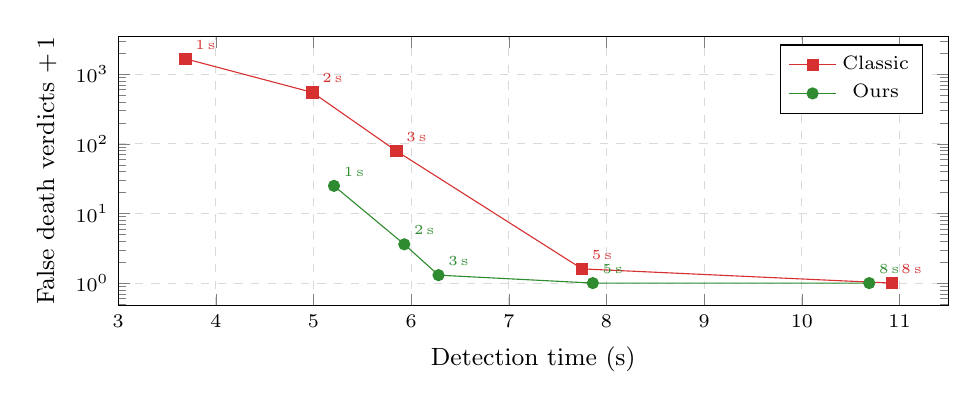
\begin{tikzpicture}
\begin{axis}[
  width=\columnwidth, height=5cm,
  xlabel={Detection time (s)}, ylabel={False death verdicts $+\,1$},
  ymode=log, xmin=3, xmax=11.5,
  legend style={font=\scriptsize, at={(0.97,0.97)}, anchor=north east},
  tick label style={font=\scriptsize}, label style={font=\small},
  grid=major, grid style={dashed, gray!30},
  nodes near coords, point meta=explicit symbolic,
  every node near coord/.append style={font=\tiny, anchor=south west}]
\addplot[color=loss, mark=square*] coordinates {
  (3.69,1663.5) [1\,s] (4.99,546.4) [2\,s] (5.85,78.7) [3\,s] (7.75,1.6) [5\,s] (10.92,1.0) [8\,s]};
\addlegendentry{Classic}
\addplot[color=win, mark=*] coordinates {
  (5.21,24.9) [1\,s] (5.93,3.6) [2\,s] (6.28,1.3) [3\,s] (7.86,1.0) [5\,s] (10.69,1.0) [8\,s]};
\addlegendentry{Ours}
\end{axis}
\end{tikzpicture}
\caption{Detection time against false death verdicts at 20\% loss, sweeping the suspicion timeout $T_s$ (labels). Lower and further left is better.}
\label{fig:tradeoff}
\end{figure}

Table~\ref{tab:slowdet} covers a node made 10$\times$ slower but alive: the classic detector declares it dead 8.8 times per run, and the slow node, missing its own deadlines, accuses others. The improved detector never declares it dead and cuts its accusations by 3.6$\times$.

\begin{table}[h]
\caption{One node 10$\times$ slower but alive.}
\label{tab:slowdet}
\small
\begin{adjustbox}{max width=\columnwidth}
\begin{tabular}{lcc}
\toprule
\textbf{Metric} & \textbf{Classic} & \textbf{Ours} \\
\midrule
Death verdicts about the slow node & \pmsd{8.8}{5.8} & \win{0.0} \\
Accusations made by the slow node & \pmsd{10.1}{3.1} & \win{\pmsd{2.8}{1.9}} \\
Detection time of a real crash (s) & \pmsd{6.32}{0.77} & \loss{\pmsd{7.41}{1.15}} \\
\bottomrule
\end{tabular}
\end{adjustbox}
\end{table}

Higher network latency is where the improved detector loses. Neither detector made false verdicts up to 300\,ms mean latency, but detection took 5.38\,s (classic) against 7.72\,s (ours) at 300\,ms. The ablation in Table~\ref{tab:ablation-det} attributes this to phi-accrual probing, whose per-peer timeouts grow with latency, and shows that agreement-based suspicion alone produces almost all of the reduction in false verdicts. Self-doubt changed false verdicts by less than one standard deviation in every test and is therefore off by default.

\begin{table}[h]
\caption{Detector ablation: false death verdicts (FD) and detection time (s).}
\label{tab:ablation-det}
\small
\begin{adjustbox}{max width=\columnwidth}
\begin{tabular}{lcccc}
\toprule
 & \multicolumn{2}{c}{\textbf{20\% loss}} & \textbf{200\,ms} & \textbf{Slow node} \\
\textbf{Detector} & FD & Time & Time & FD \\
\midrule
Classic & 77.7 & 5.85 & 5.65 & 10.6 \\
Phi only & 79.5 & 5.32 & 7.25 & 11.1 \\
Self-doubt only & 88.0 & 5.24 & 5.69 & 9.0 \\
Agreement only & 0.1 & 6.18 & 6.00 & 0.0 \\
Agreement + phi (ours) & 0.3 & 6.28 & 7.63 & 0.0 \\
Ours + self-doubt & 0.5 & 6.38 & 7.63 & 0.0 \\
\bottomrule
\end{tabular}
\end{adjustbox}
\end{table}

These results address \textbf{RQ}$_1$: false death verdicts fall by one to two orders of magnitude, at the price of detection that is 0.4--1.1\,s slower under loss and up to 2.3\,s slower under high latency.

\subsubsection{Tail latency.} With one node 10$\times$ slower (Table~\ref{tab:slow}), the classic store's median is unaffected but its tail is not: about 10\% of requests are coordinated by the slow node, and some reads wait for it. Routing by recent latency avoids it as coordinator and as replica, bringing $p_{99}$ from 1338\,ms to 210\,ms and failed requests from 2.61\% to 0.02\%. This answers \textbf{RQ}$_2$.

\begin{table}[h]
\caption{Client latency (ms) and failed requests with one node 10$\times$ slower.}
\label{tab:slow}
\small
\begin{adjustbox}{max width=\columnwidth}
\begin{tabular}{lcccc}
\toprule
\textbf{System} & $p_{50}$ & $p_{95}$ & $p_{99}$ & \textbf{Failed} \\
\midrule
Classic & \pmsd{167.4}{0.5} & \pmsd{199.2}{0.9} & \pmsd{1337.7}{18.1} & 2.61\% \\
Ours & \loss{\pmsd{171.0}{0.0}} & \win{\pmsd{198.1}{0.3}} & \win{\pmsd{209.6}{0.5}} & \win{0.02\%} \\
\bottomrule
\end{tabular}
\end{adjustbox}
\end{table}

\subsubsection{Load balance.} Table~\ref{tab:load} reports the busiest node's work relative to the average. With zipf-skewed keys ($s = 1.2$), the classic store's busiest node carries 1.68$\times$ the average; ours stays within the cap. When one key suddenly receives half of all traffic, the classic store never brings its busiest node within the cap, and the other keys' $p_{99}$ suffers because they share those nodes. Ours lends the key to extra replicas, is balanced 5.2\,s after the surge, and keeps the other keys' $p_{99}$ unchanged. No configuration produced a stale read.

\begin{table}[h]
\caption{Busiest node over average load ($\alpha = 1.25$), time to stay within the cap, and $p_{99}$ of the other keys.}
\label{tab:load}
\small
\begin{adjustbox}{max width=\columnwidth}
\begin{tabular}{lcc}
\toprule
\textbf{Metric} & \textbf{Classic} & \textbf{Ours} \\
\midrule
Zipf keys: busiest / average & 1.68 & \win{1.15} \\
Viral key: busiest / average & 2.25 & \win{1.16} \\
Viral key: within cap after (s) & never & \win{\pmsd{5.2}{0.4}} \\
Viral key: $p_{99}$ of other keys (ms) & \pmsd{283.1}{52.2} & \win{\pmsd{207.4}{0.5}} \\
\bottomrule
\end{tabular}
\end{adjustbox}
\end{table}

\subsubsection{Overhead.} At normal load without faults, hedging never fired and the improved store sent 24\% fewer messages (102.2k against 134.6k), because a read asks $R$ replicas instead of $N$. The price is latency: waiting for two chosen replicas instead of the fastest two of three adds about 5\,ms at $p_{50}$ (170.2 against 164.9\,ms) and 8\,ms at $p_{99}$ (207.6 against 199.5\,ms).

\subsubsection{Ablation.} Table~\ref{tab:ablation-req} adds the routing mechanisms one at a time. Hedging alone barely helps with a slow node and makes the viral key worse, because asking only $R$ replicas concentrates reads on the first owners. Latency-aware choice is what removes the slow-node tail; hot-key replicas are what balance the viral key; the load cap adds little on top.

\begin{table}[h]
\caption{Routing ablation.}
\label{tab:ablation-req}
\small
\begin{adjustbox}{max width=\columnwidth}
\begin{tabular}{lccc}
\toprule
 & \textbf{Slow node} & \multicolumn{2}{c}{\textbf{Viral key}} \\
\textbf{Routing} & $p_{99}$ (ms) & Busiest/avg & Others $p_{99}$ \\
\midrule
Classic & 1337.7 & 2.25 & 283.1 \\
Hedging only & 1025.1 & 3.04 & 251.9 \\
+ latency-aware choice & 209.6 & 2.14 & 208.0 \\
+ load cap & 209.6 & 1.95 & 206.8 \\
+ hot-key replicas (ours) & 209.6 & 1.16 & 207.4 \\
\bottomrule
\end{tabular}
\end{adjustbox}
\end{table}

Together with the overhead results, this answers \textbf{RQ}$_3$. Table~\ref{tab:summary} summarizes all comparisons.

\begin{table}[h]
\caption{Summary against the classic store using a colour code: \win{$\blacksquare$} = better, \tie{$\blacksquare$} = no difference, \loss{$\blacksquare$} = worse.}
\label{tab:summary}
\small
\begin{adjustbox}{max width=\columnwidth}
\begin{tabular}{lc}
\toprule
\textbf{Test} & \textbf{Ours vs classic} \\
\midrule
False death verdicts under loss & \win{77.7 $\rightarrow$ 0.3 (20\%)} \\
Slow node declared dead & \win{8.8 $\rightarrow$ 0} \\
Detection time, clean network & \loss{+0.45\,s} \\
Detection time, 300\,ms latency & \loss{+2.3\,s} \\
$p_{99}$ with a slow node & \win{1338 $\rightarrow$ 210\,ms} \\
Busiest node, viral key & \win{2.25 $\rightarrow$ 1.16$\times$} \\
Messages at normal load & \win{$-$24\%} \\
Latency at normal load & \loss{+5--8\,ms} \\
Stale reads & \tie{0 in both} \\
\bottomrule
\end{tabular}
\end{adjustbox}
\end{table}

\section{Conclusions and Future Work}

This work addresses two weaknesses of Dynamo-style stores: failure detection with fixed timeouts, and request handling that ignores speed and load. We built a complete Dynamo-style store in a deterministic simulator and replaced both parts using information nodes already exchange.

The evaluation shows that agreement-based suspicion removes almost all false death verdicts under packet loss and for slow nodes, and detects real crashes 1.5\,s sooner than a classic detector tuned to the same accuracy (\textbf{RG}$_1$). Latency-aware routing cuts $p_{99}$ with a slow node from 1338\,ms to 210\,ms (\textbf{RG}$_2$), and hot-key replicas keep the busiest node within 1.16$\times$ the average under a sudden hot key while sending 24\% fewer messages and producing no stale reads (\textbf{RG}$_3$).

\textbf{Limitations and future directions.} All results come from simulation, with a network model and a workload of our choosing; the thresholds ($m$, $K$, $\theta$, the hedge delay) were set by hand and checked against the same tests, so the numbers are tuned to them. Phi-accrual probing slows detection under high latency without a measured benefit beyond the slow-node case, and self-doubt gave no measurable benefit in our fault model, which, unlike Lifeguard's, varies the network rather than CPU load. The improved store also costs 5--8\,ms per request when nothing is wrong. Future work should rework or remove phi probing, add runtime ring membership changes, and validate the results on real machines with real traces.

\bibliographystyle{ACM-Reference-Format}
\bibliography{references}

\end{document}
